\subsubsubsubsection{Crossroads director}
\begin{figure}[h]
\centering
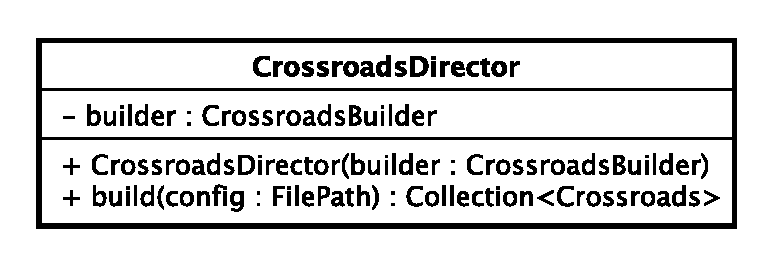
\includegraphics[scale=0.6,keepaspectratio]{images/solution/app/backend/crossroads_director.eps}
\caption{\pReactiveBuild::CrossroadsDirector}
\label{fig:sd-app-crossroads_director}
\end{figure}
\FloatBarrier
\begin{itemize}
  \item \textbf{\descr} \\
    It represents the concrete director of the crossroads builder.
    \item \textbf{\attrs}
  \begin{itemize}
    \item \texttt{builder: CrossroadsBuilder} \\
The builder object which builds parts of the district.
  \end{itemize}
  \item \textbf{\ops}
  \begin{itemize} 
    \item[+] \texttt{CrossroadsDirector(builder: CrossroadsBuilder)} \\
Creates a concrete crossroads director with its own crossroads builder.
    \item[+] \texttt{build(config: FilePath) : Collection<Crossroads>} \\
Builds a collection of crossroads according to the configuration file. 
It uses the builder multiple times 
to create incrementally a configuration of the requested crossroads as specified
in the configuration file. 
  \end{itemize}
\end{itemize}
